\begin{ndef}{: Diameter}
	We define the \emph{\textbf{diameter}} of the set as:
	\begin{equation*}
		\text{diam}(\mc{S})=\sup\{d(x,y)\st x,y\in\mc{S}\}
	\end{equation*}
\end{ndef}

\begin{figure}[htbp]
	\centering
	\begin{tikzpicture}
		%\draw[thick, dotted, black, thick, fill = white!60!gray] (-1, 1) to [curve through ={(0.5,0.5)..(1,-1)..(-0.5,-0.5)}] (-1, 1);
		
		\draw[thick, dotted, black, thick, fill = white!60!gray] (0, 0.6) to [curve through ={(1.8, 0.475)..(4.75, 0.4)..(4.8, 0.02)..(5, 0)..(4.9, -0.25)..(4.75, -0.76)..(2.5, -0.72)..(0, -1)..(-1.85, -0.78)..(-1.9, -0.4)..(-2, 0)..(-1, 0.5)}] (0, 0.6);
		
		\draw[<->] (-1.65,-1.15)--(4.6,0.98);
		
		%\draw[fill] (1.3,-0.14) circle (1pt);
		
		\draw[->] (1.3,-0.14)--(1.3,-1.3);
		
		\node[below] at (1.3,-1.3) {\(d(x,y)=\text{diam}(\mc{S})\)};
		
		\node[below] at (4.3, -0.6) {\(\mc{S}\)};
	\end{tikzpicture}
	
	\caption{Visualization of the diameter.}
\end{figure}

\begin{ntheorem}{: Cantor's intersection theorem}
	Let \((\mc{X},d)\) be a metric space; the following are equivalent:
	\begin{enumerate}[(a)]
		\item \((\mc{X},d)\) is complete -- every Cauchy sequence converges in \(\mc{X}\).
		
		\item For every sequence of nested, closed, and non-empty sets \(\mc{F}_1\supseteq\mc{F}_2\supseteq\mc{F}_3\supseteq\dots\) in \(\mc{X}\) having \(\text{diam}(\mc{F}_n)\to 0\) as \(n\to\infty\); the set \(\mc{F}=\displaystyle\bigcap_{n=1}^{\infty}\mc{F}_n\) contains exactly one point.
	\end{enumerate}
\end{ntheorem}

\begin{proof}
	(a\(\Rightarrow\)b) Givens sets \((\mc{F}_n)\) as in setup (b). Pick any \(x_n\in\mc{F}_n\) for each \(n\), this defining a sequence \((x_n)\); this sequence is Cauchy: let \(\eps>0\) be given. We use the fact that \(\text{diam}(\mc{F}_n)\to 0\) to get \(N\in\N\) such that \(\text{diam}(\mc{F}_n)<\eps\) for all \(n>N\). In our sequence, if \(m,n>N\), then both \(x_m,x_n\in\mc{F}_{\min\{m,n\}}\subseteq\mc{F}_{N+1}\); hence \(d(x_m,x_n)<\eps\). By completeness, some \(\hat{x}\in\mc{X}\) satisfies \(\hat{x}=\displaystyle\lim_{n\to\infty}x_n\). Note that:
	\begin{enumerate}[(i)]
		\item \(\hat{x}\in\mc{F}\), because for each \(n\), \emph{closed set} \(\mc{F}_n\) contains each point \(x_{n+p}\) for \(p\in\N\), so \(\hat{x}=\displaystyle\lim_{p\to\infty}x_{n+p}\) lies in \(\mc{F}_n\).
		
		\item If \(y\neq\hat{x}\), then \(y\notin\mc{F}\), because if \(y\neq\hat{x}\), then \(d(y,\hat{x})>0\); however, \(\mc{F}\subseteq\mc{F}_n\subseteq\B[\hat{x};\text{diam}(\mc{F}_n))\). Hence, \(y\in\mc{F}\) is excluded by the fact that \(\text{diam}(\mc{F})\to 0\). 
	\end{enumerate}
	This tells us that \(\mc{F}=\hat{x}\).
	
	\medskip
	
	(b\(\implies\)a) Given a Cauchy sequence \((x_n)\) in \(\mc{X}\), let 
	\begin{equation*}
		\mc{F}_n=\ol{\{x_n,x_{n+1},x_{n+2},\dots\}}.
	\end{equation*}
	Now, each \(\mc{F}_n\) is closed, non-empty, and \(\mc{F}_n\supseteq\mc{F}_{n+1}\). Furthermore, \(\text{diam}(\mc{F}_n)\to 0\) as \(n\to\infty\), since \((x_n)\) is Cauchy: let \(\eps>0\) be given; we get \(N\in\N\) such that for all \(m,n>N\), we have \(d(x_m,x_n)<\eps\). This makes \(\text{diam}(\mc{F}_n)\leq\eps\) for all \(n\in\N\), so using (b), let \(\{\hat{x}\}=\displaystyle\bigcap_{n\in\N}\mc{F}_n\). We show that \(x_n\to\hat{x}\): given any \(\eps>0\), we pick a sufficiently large \(N\) such that \(\text{diam}(\mc{F}_n)<\eps\) for all \(n>N\); then \(x_n,\hat{x}\in\mc{F}_n\) which tells us that \(d(x_n,\hat{x})<\eps\).
\end{proof}

\begin{figure}[htbp]
	\centering
	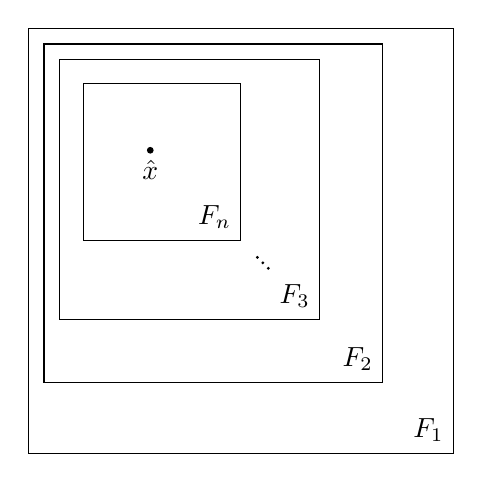
\begin{tikzpicture}
		\draw[] (2.7, 2.7) -- (-2.7, 2.7) -- (-2.7, -2.7) -- (2.7, -2.7) -- (2.7, 2.7);
		\draw[] (-2.3, -1) -- (-2.3, 2.3) -- (1, 2.3) -- (1, -1) -- (-2.3, -1);
		\draw[] (-2.5, -1.8) -- (-2.5, 2.5) -- (1.8, 2.5) -- (1.8, -1.8) -- (-2.5, -1.8);
		\draw[] (-2, 0) -- (-2, 2) -- (0, 2) -- (0, 0) -- (-2, 0);
		\draw[-, dotted, thick] (0.2,-0.2)--(0.4,-0.4);
		%\draw[dotted, thick, fill = white!60!lightgray] (-1.15, 1.15) circle (25pt);
		\draw[fill] (-1.15, 1.15) circle (1pt);
		\node[below] at (-1.15, 1.15) {\(\hat{x}\)};
		%\node[right] at (-1.1, 1.7) {\(\mc{U}\)};
		\node[left] at (2.7, -2.4) {\(\mc{F}_1\)};
		\node[left] at (1.8, -1.5) {\(\mc{F}_2\)};
		\node[left] at (1, -0.7) {\(\mc{F}_3\)};
		\node[left] at (0,0.3) {\(\mc{F}_n\)};
	\end{tikzpicture}
	\caption{Visualization of the theorem.}
\end{figure}

\subsection{Completing a metric space}
Let \((\mc{X},d)\) be a metric space. We can construct a \emph{\textbf{complete}} metric space \((\hat{\mc{X}},D)\) such hat \(\mc{X}\) is dense in \((\hat{\mc{X}},D)\), and \(D(x,y)=d(x,y)\) for all \(x,y\in\mc{X}\).

\begin{note}[Analogy]
	We built \(\R\) from \(\Q\) by exactly these methods \((\R=\hat{\Q})\).
\end{note}
\begin{note}[``Weasel words"]
	\((\hat{\mc{X}},D)\) actually contains a ``working copy" of \((\mc{X},d)\)\dots not the exact points.
\end{note}
\subsubsection*{Outline of the process}
Let \(\text{CS}(\mc{X})\) be the set of all Cauchy sequences \(a=(a_1,a_2,\dots)\) with elements in \(\mc{X}\); we will call them ``vectors". Elements of \(\hat{\mc{X}}\) will be sets like this:
\begin{equation*}
	P[a]=\left\{b\in\operatorname{CS}(\mc{X})\st \lim_{n\to\infty}d(a_n,b_n)=0\right\}.
\end{equation*}
Observe:
\begin{enumerate}[(i)]
	\item Every \(a\in\operatorname{CS}(\mc{X})\) lies in \(P[a]\).
	
	\item For given \(a,b\in\operatorname{CS}(\mc{X})\), the sets \(P[a],P[b]\) are either disjoint or equal.
	
	\item Different ``representatives" \(a,b\in\operatorname{CS}(\mc{X})\) can give the same \(P[a]=P[b]\) in \(\hat{X}\).
\end{enumerate}
\begin{example}
	If \(\mc{X}=\Q\), observe that \(a=(0,0,0,\dots)\) and \(b=\left(1,\displaystyle\frac{1}{2},\frac{1}{3},\frac{1}{4},\dots\right)\) have \(P[a]=P[b]\).
\end{example}
The metric in \(\hat{\mc{X}}\) is defined as: if \(P[a],P[b]\in\hat{\mc{X}}\), let 
\begin{equation*}
	D\left(P[a],P[b]\right)=\lim_{n\to\infty}d(a_n,b_n).
\end{equation*}
Things to check:
\begin{enumerate}[(i)]
	\item This limit actually exists:
	\begin{equation*}
		\text{Show}~\delta_n=d(a_n,b_n)~\text{is Cauchy in}~\R.
	\end{equation*}
	
	\item Different representatives \(a'\in P[a]\), \(b'\in P[b]\) give the same \(\displaystyle\lim_{n\to\infty}d(a_n',b_n')\).
	
	\item \(D(\cdot,\cdot)\) is truly a metric on \(\hat{\mc{X}}\).
	
	\item \(\mc{X}\) -- or a suitable copy -- is dense in \(\hat{\mc{X}}\); we use constant sequences for this.
\end{enumerate}